
%(BEGIN_QUESTION)
% Copyright 2011, Tony R. Kuphaldt, released under the Creative Commons Attribution License (v 1.0)
% This means you may do almost anything with this work of mine, so long as you give me proper credit

This conveyor belt control circuit has a problem.  The siren energizes when the ``Start'' pushbutton is pressed, but the conveyor belt never moves.  The siren remains energized until the ``Stop'' button is pressed.  A technician begins diagnosing the circuit, following the steps shown (in order).  His first action is to press the ``Start'' switch so that the siren is continuously activated, before he begins any diagnostic tests:

$$\includegraphics[width=15.5cm]{i03531x01.eps}$$

\begin{itemize}
\item{} {\bf Test 1:} Measured 120 VAC between points {\bf A} and {\bf E}.
\vskip 25pt
\item{} {\bf Test 2:} Measured 120 VAC between points {\bf N} and {\bf L}.
\vskip 25pt
\item{} {\bf Test 3:} Measured 0 VAC between points {\bf J} and {\bf K}.
\vskip 25pt
\item{} {\bf Test 4:} Measured 0 VAC between points {\bf D} and {\bf M}.
\vskip 25pt
\item{} {\bf Test 5:} Measured 120 VAC between points {\bf A} and {\bf D}.
\vskip 25pt
\medskip

Identify any useful information about the nature or location of the fault derived from the results of each test, in order of the tests performed.  If the test is not useful (i.e. provides no new information), mark it as such.  Assuming there is only one fault in the circuit, identify the location and nature of the fault as precisely as you can from the test results shown above.

\vfil 

\underbar{file i03531}
\eject
%(END_QUESTION)





%(BEGIN_ANSWER)

\begin{itemize}
\item{} {\bf Test 1:} Measured 120 VAC between points {\bf A} and {\bf E}.  {\it This is an unnecessary test, as we already know there is 120 VAC power available to the control circuit (otherwise, the siren would never energize).}
\vskip 5pt
\item{} {\bf Test 2:} Measured 120 VAC between points {\bf N} and {\bf L}.  {\it This confirms the time-delay relay coil is receiving power, limiting the fault to either an ``open'' TD1 coil, or an ``open'' somewhere between points B and M.}
\vskip 5pt
\item{} {\bf Test 3:} Measured 0 VAC between points {\bf J} and {\bf K}.  {\it This is an unnecessary test, as we already know NC contact M1 is closed, because the siren is being energized.}
\vskip 5pt
\item{} {\bf Test 4:} Measured 0 VAC between points {\bf D} and {\bf M}.  {\it This proves no power is getting to the M1 contactor coil, indicating an ``open'' fault somewhere between B and M other than the coil itself.}
\vskip 5pt
\item{} {\bf Test 5:} Measured 120 VAC between points {\bf A} and {\bf D}.  {\it This test alone proves an ``open'' fault must exist between points A and D.  Combined with knowledge that the siren is latching on, we know the ``open'' fault cannot lie between A and B, and therefore must lie somewhere between B and D.}
\end{itemize}

\vskip 10pt

{\bf The fault is an ``open,'' either between B and contact TD1, at contact TD1 itself, or between points C and D.}

%(END_ANSWER)





%(BEGIN_NOTES)


%INDEX% Troubleshooting review: electric circuit diagnostic test rationale

%(END_NOTES)


